\documentclass[a4paper,11pt]{article}
\usepackage{exptech}
\usepackage{textcomp}
\usepackage{graphicx}
\usepackage{array}
\usepackage[babel=true]{csquotes}
\usepackage{url}
\usepackage{hyperref}
\usepackage{wrapfig}
\usepackage[export]{adjustbox}
\usepackage{titletoc}
\usepackage{array}

\hypersetup{
  pdftitle={Systèmes hétérogènes - Technologie RAID}, % title
  pdfnewwindow=true, % links in new window
  colorlinks=true, % false: boxed links; true: colored links
  linkcolor=black, % color of internal links (change box color with linkbordercolor)
  citecolor=cyan, % color of links to bibliography
  filecolor=cyan, % color of file links
  urlcolor=cyan % color of external links
}

\title{
  \textbf{Systèmes hétérogènes}\\
  Technologies RAID
}
\markright{Avalon - Rapport de pré-étude}
\author{
\begin{minipage}{0.4\textwidth}
	\begin{flushleft} \large
		\emph{Auteurs :}\\
                Amin \textsc{Nasseh}\\
		Alexandre \textsc{Leonardi}\\
	\end{flushleft}
\end{minipage}
\begin{minipage}{0.4\textwidth}
	\begin{flushright} \large
		\emph{Encadrant :} \\
		Roland \textsc{Agopian}\\
	\end{flushright}
\end{minipage}
}

\date{\today}

\begin{document}
\maketitle
\thispagestyle{empty}
\begin{abstract}
RESUME ICI
\end{abstract}
\pagebreak

\tableofcontents
\pagebreak


\section{Introduction}

\pagebreak
\section{Mécanisme de démarrage d'un PC}
\pagebreak
\section{Mécanisme de démarrage d'un système Linux}
\pagebreak
\section{Procédure de modification de mot de passe root sous Linux}
On trouve différentes solutions sur le net permettant d'arriver à cette solution, plus ou moins complexes de mises en \oe{}vre. En voici trois. 

\subsection{Mode utilisateur unique}
Cette méthode marche pour tout bootloader, mais nous allons supposer qu'il s'agit d'un utilisateur utilisant GRUB.

Dans un premier temps, se placer sur la ligne correspondant à votre partition de boot classique (cf \textsc{figure ~\ref{fig:grub-boot-menu}}) et appuyer sur "e" .

\begin{figure}[h!]
	\centering
		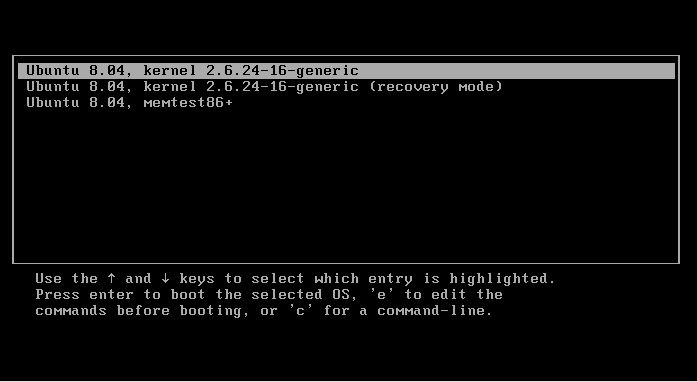
\includegraphics[width=1.00\textwidth]{boot/grub-boot-menu.png}
	\caption{Menu initial de GRUB}
	\label{fig:grub-boot-menu}
\end{figure}

Puis se déplacer vers la ligne \emph{kernel} (cf \textsc{figure ~\ref{fig:edit-grub-boot-option}}) et appuyer de nouveau sur "e" pour l'éditer. 

\begin{figure}[h!]
	\centering
		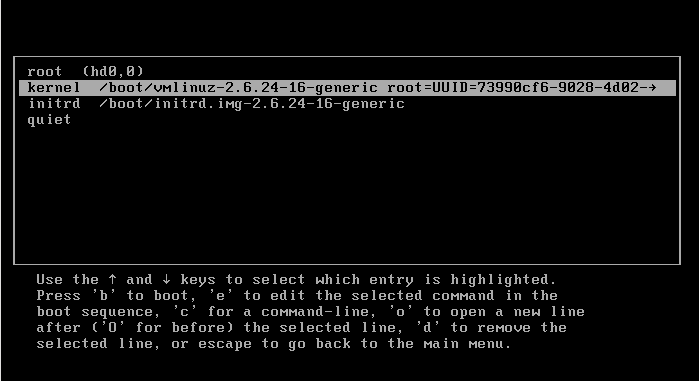
\includegraphics[width=1.00\textwidth]{boot/edit-grub-boot-option.png}
	\caption{Menu d'édition de GRUB}
	\label{fig:edit-grub-boot-option}
\end{figure}

Il suffit maintenant de rajouter \verb|single| à la fin de la ligne de commande, en prenant bien soin qu'il y ait un espace entre la fin du texte original et le début de \verb|single|. Il est possible que votre système demande le mot de passe root pour se connecter en mode utilisateur unique ; dans ce cas rajouter encore \verb|init=/bin/bash| après le \verb|single|. Appuyer sur "entrée" pour valider les modifications. 

Il suffit maintenant d'appuyer sur "b" pour booter en mode utilisateur unique et ainsi avoir accès à une invite de commande. Sur certains systèmes vous aurez besoin de monter es partitions \verb|/| et |/proc|. Pour cela entrer la commande suivante :
\verb|mount -o remount,rw / mount -o remount,rw /proc|

Entrer maintenant la commande \verb|passwd|. Le système va vous demander d'entrer un nouveau mot de passe root, puis de le confirmer (cf \textsc{figure ~\ref{fig:reset-linux-root-password}}). Il ne reste plus qu'à redémarrer et vous connecter avec le nouveau mot de passe.

\begin{figure}[h!]
	\centering
		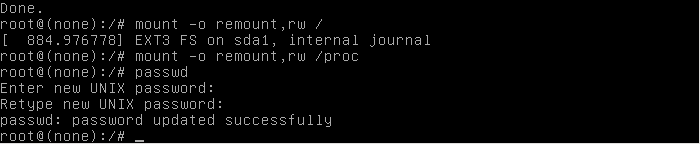
\includegraphics[width=1.00\textwidth]{boot/reset-linux-root-password.png}
	\caption{Changement de mot de passe root}
	\label{fig:reset-linux-root-password}
\end{figure}

\subsection{Démarrer sur un disque bootable}
Vous pouvez mettre en place cette solution avec le CD d'installation Linux que vous avez utilisé ou en en créant un nouveau (cela peut également être fait sur une clé USB, à l'aide par exemple de \href{http://www.linuxliveusb.com/}{Linux Live USB Creator} et d'un .iso de votre distribution Linux). Démarrer sur ce disque comme lors de l'installation du système d'exploitation.

Une fois sur un bureau, plutôt que de lancer l'installation, ouvrir une console. 

Taper \verb|mkdir mountplace| pour créer un dossier nommé "mountplace" où le disque sera plus tard monté.

Taper \verb|mount /dev/hdaX mountplace| (où X est le numéro associé à votre partition root) pour monter la partition concernée et pouvoir y accéder.

Taper \verb|cd mountplace/etc| pour vous déplacer dans le dossier etc de votre partition. 

Ouvrez le fichier \emph{shadow} avec l'éditeur de texte de votre choix, par exemple grâce à la commande \verb|vi shadow|

Il faut maintenant trouver une ligne contenant les informations de l'utilisateur root, qui devrait ressembler à \verb|root:dsfDSDF!s:12581:0:99999:7:::|. Vous allez devoir enlever la partie entre le premier et le deuxième deux-points. Avec l'exemple donné, vous obtiendriez \verb|root::12581:0:99999:7:::| (on voit que \emph{dsfDSDF!s} a disparu).

Vous pouvez maintenant sauvegarder votre modification et quitter votre éditeur de texte, taper \verb|cd| pour quitter le dossier etc, \verb|unmount mountplace| pour démonter la partition et enfin redémarrer votre ordinateur.

Prenez soin de retirer le CD ou la clé USB que vous avez utilisé avant de redémarrer. Vous n'aurez pas besoin de votre mot de passe pour vous connecter à votre compte. Pensez à en configurer un nouveau dès que possible ! 

\subsection{Monter le disque sur un autre ordinateur}
Cette dernière méthode est la plus complexe de mise en \oe{}uvre mais la plus sûre de marcher (à moins que le disque dur sur lequel votre système est installé soit encrypté, et que vous ayez oublié ce mot de passe également... ce qui confinerait à de la mauvaise volonté). 

Dans un premier temps, mettre votre ordinateur hors-tension, ouvrir le boitier et retirer le disque dur (vous pouvez laisser passer quelques secondes ou minutes après la mise hors-tension pour que les condensateurs présents dans votre machine se déchargent). 

Ensuite, brancher le disque dur sur un autre ordinateur, de préférence utilisant un système Linux aussi, car le format de fichier utilisé par Linux n'est pas reconnu par Windows et Mac. 

Une fois le second ordinateur démarré, la démarche est la même qu'avec un disque bootable :
\begin{enumerate}
	\item \verb|mkdir mountplace| pour créer un répertoire où sera monté le disque que vous avez déplacé
    \item \verb|mount /dev/hdaX mountplace| où hdaX est le nom du disque que vous avez déplacé
    \item \verb|cd mountplace/etc| pour vous déplacer dans le répertoire etc de votre disque
    \item \verb|vi shadow| (ou tout autre éditeur de texte selon votre préférence) pour ouvrir le fichier shadow
    \item localiser la ligne correspondant à l'utilisateur root, ressemblant à \verb|root:dsfDSDF!s:12581:0:99999:7:::|
    \item retirer la partie entre le premier et le deuxième deux-points, pour obtenir un résultat ressemblant à \verb|root:s:12581:0:99999:7:::|
    \item Sauvegarder la modification et quitter l'éditeur de texte
    \item \verb|cd| pour quitter le dossier etc
    \item \verb|unmount mountplace| pour démonter votre disque dur
\end{enumerate}

Une fois tout ceci fait, vous pouvez éteindre l'ordinateur, débrancher le disque dur et le rebrancher dans l'ordinateur d'origine, puis remettre ce dernier sous tension. 

Vous devriez alors pouvoir vous connecter à votre compte sans mot de passe. Là encore, pensez à renseigner un nouveau mot de passe root dès que possible. 
\pagebreak
\section{Conclusion}
Pour terminer ce rapport, il est bon de préciser que dans chacun des points abordés (démarrage d'un ordinateur jusqu'au chargement du noyau d'un OS, démarrage d'un système Linux, changement de mot de passe root sous Linux si celui-ci a été oublié), il est possible que l'explication donnée ne soit pas exhaustive. 

Cela est dû à la multiplicité des possibilités en terme de matériel et de logiciel. De fait, tout couvrir en détail représenterait un travail bien plus titanesque que ce qui est possible dans le cadre de ce projet. 

Un exemple de ce qui n'a pas été traité est le couple UEFI/GPT. UEFI (Unified Extensible Firmware Interface) est un remplaçant à la technologie BIOS dont les spécifications ont été publiées en 2005 et qui tend à être prédominant sur les nouvelles cartes mères. GPT (GUID Partition Table, GUID signifiant Globally Unique IDentifiers) est un standard de tables de partitions qui vise à remplacer MBR et fait lui-même partie du standard UEFI. 

Ces deux technologies prennent une approche différente, mais comme d'autres, les traiter ici demanderait bien trop de temps. Il reste néanmoins que le présent rapport donne une vue d'ensemble de ce qui existe et apporte un degré de compréhension non-négligeable sur la procédure de démarrage d'un ordinateur Linux. 
\pagebreak
\nocite{*}
\bibliography{root/biblio}

\end{document}
